\documentclass[a4paper]{article}
\usepackage[fontset=fandol]{ctex}
\usepackage[margin=1.65cm]{geometry}
\usepackage{amsmath,amssymb}
\usepackage{graphicx}
\usepackage{hyperref}
\usepackage{longtable,booktabs}
\usepackage{xcolor}
\usepackage{enumitem}
\usepackage{listings}
\lstset{basicstyle=\ttfamily\small,breaklines=true,columns=fullflexible,keepspaces=true}
\hypersetup{colorlinks=true,linkcolor=blue,urlcolor=blue}
\setlist[itemize]{leftmargin=1.25em,itemsep=0.18em}
\setlength{\parskip}{0.45em}
\setlength{\parindent}{2em}
\sloppy
\title{第 01 讲：课程全景与 tokenization}
\author{CS336 Spring 2026 public videos and official course materials}
\date{}
\begin{document}
\maketitle
\tableofcontents
\newpage
\section{本章导读}
本章讨论 \textbf{课程全景与 tokenization}。CS336 的第一层目标不是把现成大模型当作黑箱使用，而是把 language model 从输入文本、训练目标、模型结构、数据、系统和评估这些部件重新拆开。只有拆开之后，读者才能判断一个设计选择究竟改变了什么。
设想你要复现实验室里一个 7B language model（语言模型）的最小训练栈：你不能只下载 tokenizer，也不能只调用框架默认配置，而要解释为什么同一段 Unicode 文本会变成某个 token 序列，为什么这个序列长度会改变训练成本，以及为什么课程要把 tokenizer、architecture、data 和 systems 放在同一个问题里。
本章对应 CS336 Spring 2026 第 01 个公开视频，并结合课程页提供的可解析资料。视频和课程页给出事实边界；正文把这些材料改写为可自学的教材章节。
阅读本章时，先理解问题为什么存在，再看定义、公式和实现形态，随后通过例题和练习检查自己是否能独立复现这条 reasoning chain。
\begin{figure}[h]
\centering
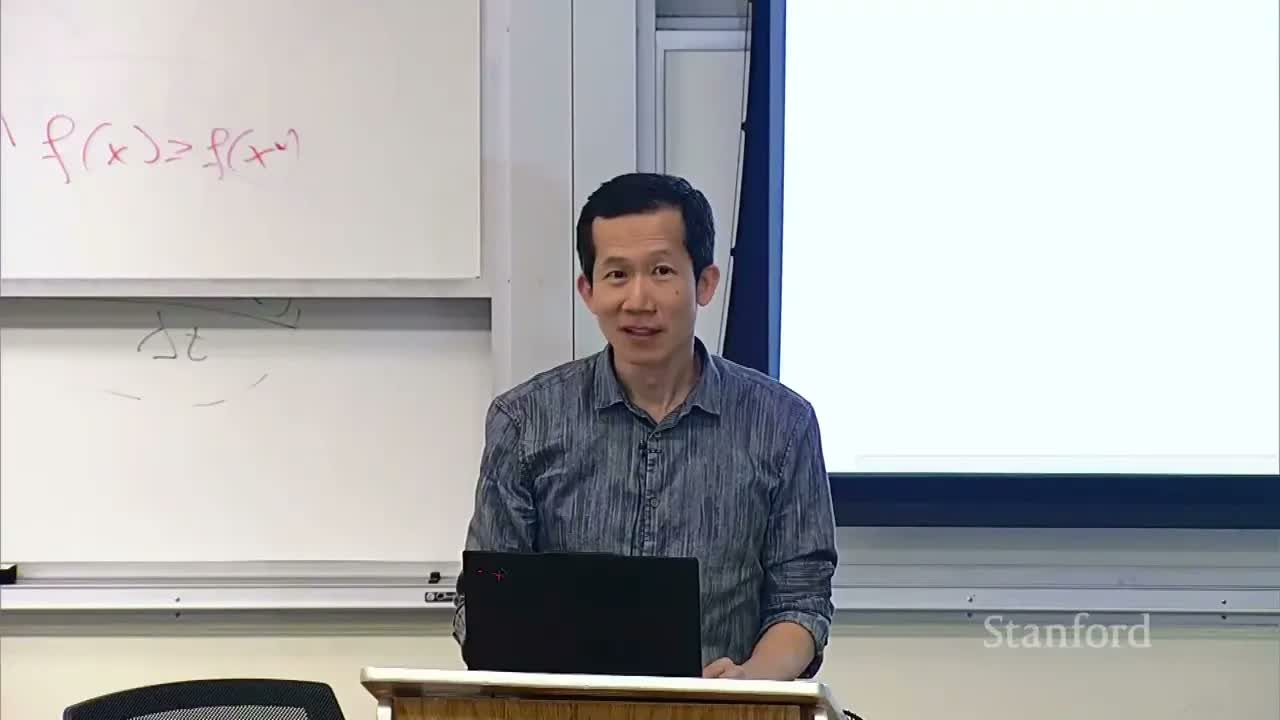
\includegraphics[width=0.58\linewidth]{source_anchor.jpg}
\caption{第 01 讲的课程图像锚点。}
\end{figure}
\subsection{本章知识路线}
\begin{itemize}
\item 本章首先说明 课程全景与 tokenization 为什么是 language modeling pipeline 中不可跳过的一环。
\item 其次定义本章反复使用的术语，并说明这些术语对应的计算对象或系统对象。
\item 随后用公式和伪代码表达主要机制，让概念能够落到可计算的变量上。
\item 最后给出例题、风险讨论和练习，便于读者检查自己是否真正掌握了机制。
\end{itemize}
\subsection{结构图}
下面的图用于帮助读者定位本章的核心结构。先看概念之间的依赖，再回到正文中的公式、伪代码和例题。
\begin{figure}[h]
\centering
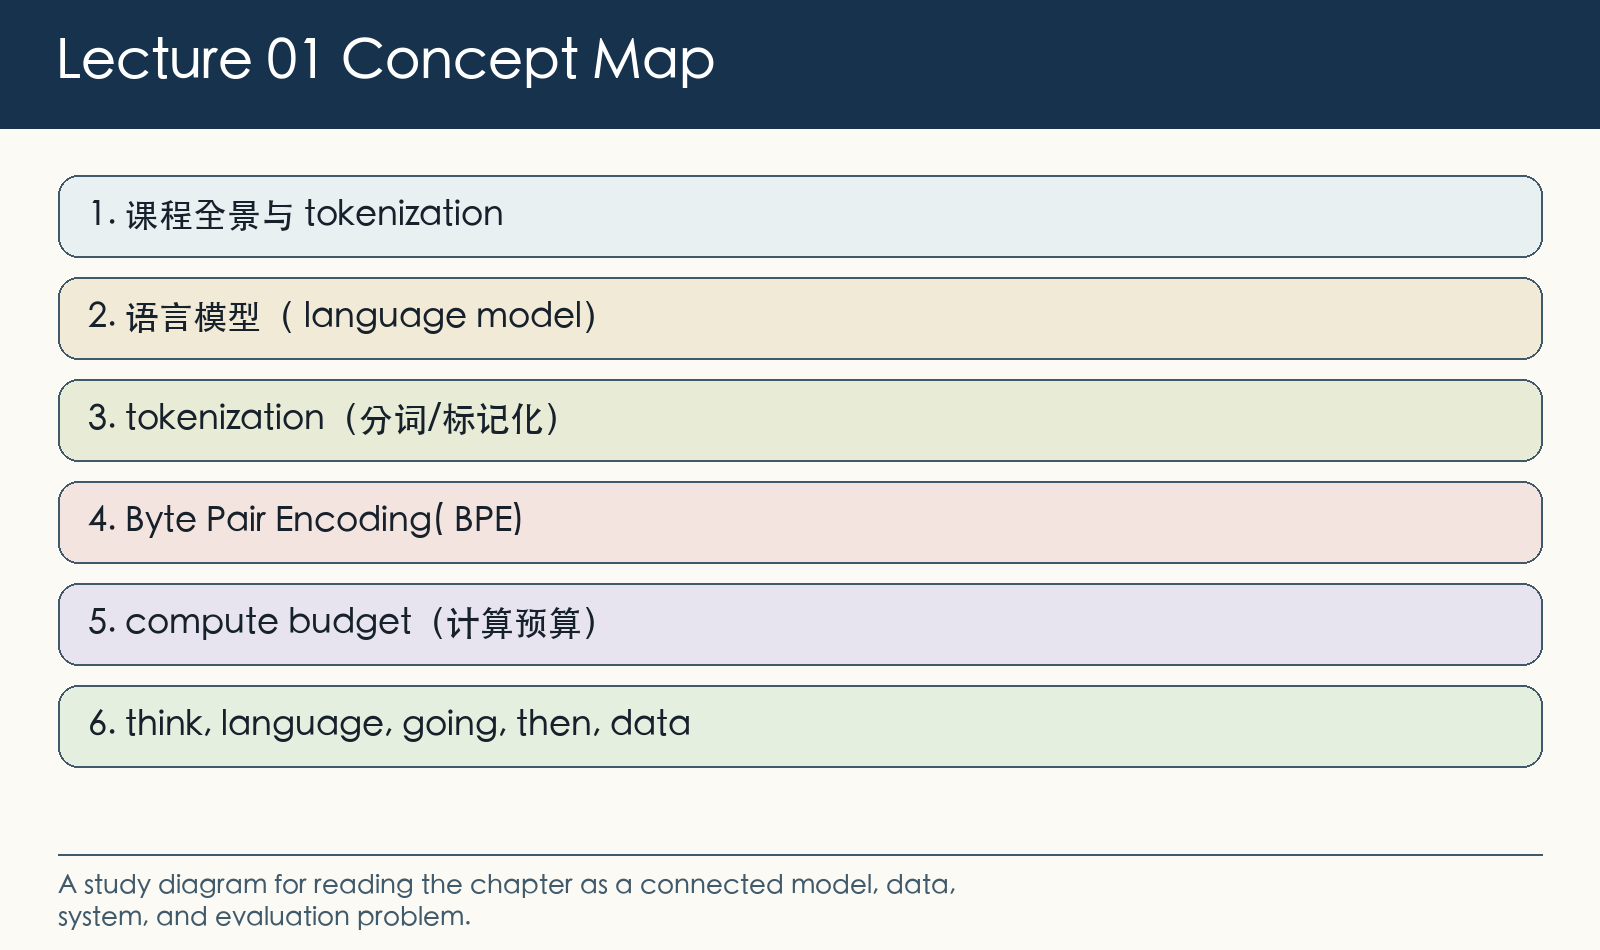
\includegraphics[width=0.72\linewidth]{figures/source_grounded_concept_map.png}
\caption{第 01 讲概念图：本章问题、术语和机制的关系。}
\end{figure}
\begin{figure}[h]
\centering
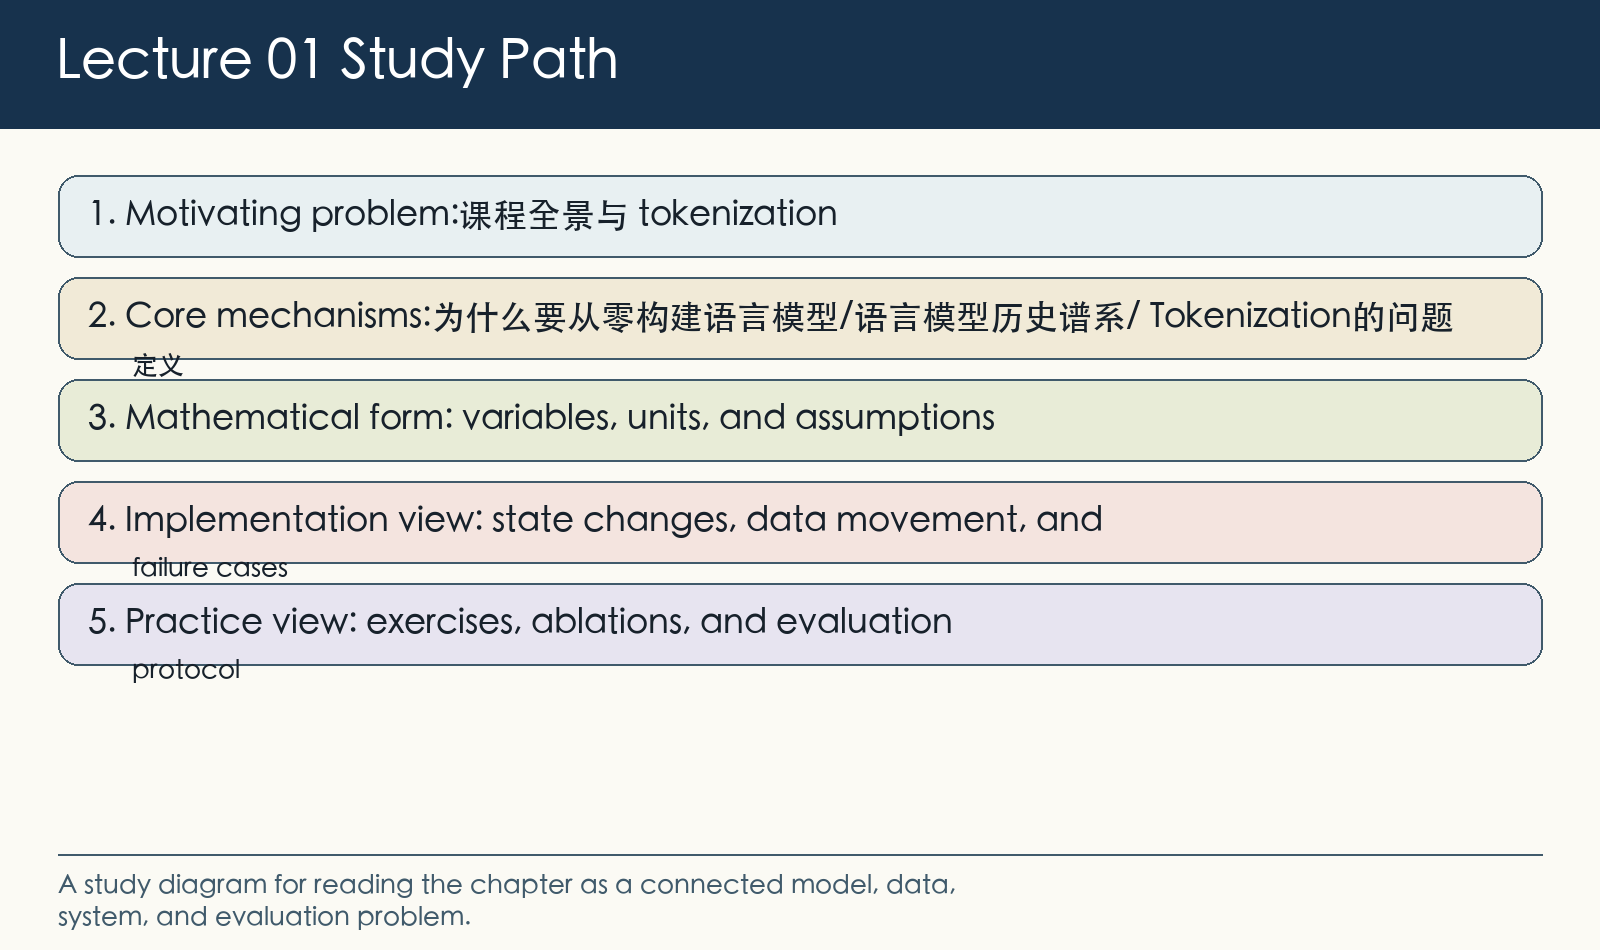
\includegraphics[width=0.72\linewidth]{figures/source_grounded_checklist.png}
\caption{第 01 讲学习路径：从问题定义进入公式、实现、实验和练习。}
\end{figure}
\section{本章主线}
课程全景与 tokenization 的主线是从一个可观察的问题出发，逐步引出表示、目标、实现和实验。读者应把每个机制放回 language modeling pipeline 的位置。
\subsection{本章要解决的核心问题}
本讲的主线是解释为什么 CS336 要坚持 from scratch。课程不是让学生背诵最新模型名字，而是把 tokenizer、architecture、optimizer、data、systems、evaluation 和 post-training 放在同一个可执行栈里理解。
读完这一段后，应能用一两句话说明 课程全景与 tokenization 要解决的瓶颈，并指出这个瓶颈发生在数据、模型、优化、系统还是评估层。
\subsection{从机制到资源账本}
tokenization 是第一个技术入口：任何语言模型都不能直接处理字符串，而要先把 Unicode 文本变成 token 序列。tokenizer 的选择会改变序列长度、训练 token 统计、attention 成本和下游语言覆盖。
随后把机制写成账本：输入规模是什么，主要状态是什么，成本或质量指标怎样随变量改变。这个账本让后面的公式不再只是符号。
\subsection{从课堂讲解到可复现实验}
课程反复强调 mechanics、mindset、intuition 的区别：mechanics 可以通过实现获得，mindset 是计算和数据账本意识，intuition 则依赖实验并且不总能从小模型迁移到 frontier 模型。
最后把课堂讲解转成可复现实验：固定协议，改变一个变量，记录中间量，并解释结果为何支持或反驳原来的机制判断。
\section{术语、符号与问题边界}
本章的术语横跨模型、数据和系统。读者需要先知道每个词指向的对象：有些词描述数学目标，有些词描述张量形状，有些词描述硬件瓶颈，还有一些词描述评估协议。术语边界不清，后面的公式和实现就会变成空洞的缩写。
\begin{longtable}{p{0.08\linewidth}p{0.42\linewidth}p{0.42\linewidth}}
\toprule
\textbf{\#} & \textbf{术语} & \textbf{阅读要求}\\
\midrule
1 & 语言模型（language model） & 给出定义、一个最小例子、一个关联公式或代码位置，以及一个典型失败情形。\\
2 & tokenization（分词/标记化） & 说明它如何改变训练样本或 token 分布，并给出一个会改变结论的数据边界条件。\\
3 & Byte Pair Encoding (BPE) & 给出定义、一个最小例子、一个关联公式或代码位置，以及一个典型失败情形。\\
4 & compute budget（计算预算） & 把它放入资源账本：单位是什么，随输入规模怎样变化，最容易被哪类 benchmark 误读。\\
5 & from-scratch philosophy（从零构建哲学） & 给出定义、一个最小例子、一个关联公式或代码位置，以及一个典型失败情形。\\
\bottomrule
\end{longtable}
这些术语之间有依赖关系。例如 tokenization 改变 sequence length，sequence length 又改变 attention FLOPs、KV cache 和 evaluation token budget；parallelism 改变显存占用，也改变通信瓶颈和故障恢复方式。
\subsection{术语之间的关系}
在本章中，语言模型（language model） 给出问题入口，tokenization（分词/标记化） 描述主要机制，Byte Pair Encoding (BPE) 则把机制连接到可测量的结果。读教材时应当沿着这个链条追问：输入是什么，中间状态怎样改变，输出指标为什么随之变化。
课程材料还会反复出现 data、e.g.、scaling、compute、scale、training 等词。它们不是一组同义标签，而是提示本章的不同层次：有的指对象，有的指操作，有的指约束或指标。
因此，术语表不是背诵清单，而是后文阅读的索引。遇到一个术语时，先定位它属于 representation、optimization、systems、data 还是 evaluation，再判断它改变哪一项账本。
\section{为什么要从零构建语言模型}
本节讨论 为什么要从零构建语言模型。它先限定 课程全景与 tokenization 要回答的基本问题：哪些现象需要解释，哪些变量可以测量，哪些结论必须回到 输入规模、资源使用、指标变化和失败模式 中检验。
\subsection{课程目标与问题边界}
课程把语言模型当作一整套技术栈，而不是只把 API prompt 当作抽象接口；视频开场强调研究者需要理解底层 mechanics、mindset 和 intuition。
课程材料把课程目标表述为 understanding via building，并把数据、architecture、training、systems、evaluation、post-training 串成一条端到端路径。
学习这门课时应把每个组件放回 budget 约束：同样资源下，算法效率、数据质量和系统效率共同决定最终模型。
为什么要从零构建语言模型 为 课程全景与 tokenization 提供一个局部观察点。接下来要把定义、公式、实现和实验条件连成同一条解释链。
\subsection{为什么要从零构建语言模型 的机制}
课程把语言模型当作一整套技术栈，而不是只把 API prompt 当作抽象接口；视频开场强调研究者需要理解底层 mechanics、mindset 和 intuition。 在 为什么要从零构建语言模型 中，核心对象是模型、数据或实验状态。本节把这些对象从口头描述转成可定义、可实现和可检查的机制。
课程材料把课程目标表述为 understanding via building，并把数据、architecture、training、systems、evaluation、post-training 串成一条端到端路径。 因而同一个方法在不同规模下可能改变不同的变量，尤其是输入规模、资源使用、指标变化和失败模式。比较方法时，必须同时给出问题规模和实验条件。
学习这门课时应把每个组件放回 budget 约束：同样资源下，算法效率、数据质量和系统效率共同决定最终模型。 可检验性来自清楚的变量、可复现的程序和能被反例挑战的结论。
因此，为什么要从零构建语言模型 的学习目标是把 课程全景与 tokenization 中的局部机制讲到可以实现、测试和反驳的程度。
\subsection{资源、效率与效果的关系}
\[\text{accuracy} \approx \text{algorithmic efficiency} \times \text{resources}\]
符号说明：resources 表示可用算力、数据和工程时间；algorithmic efficiency 表示在相同资源下把 loss 或 benchmark score 推向更优的能力。
这个关系式给出 为什么要从零构建语言模型 的最小数学结构。读者应检查变量单位、取值范围和可观测性；如果某个量只能间接估计，就必须说明 proxy。
任何 proxy 都只测量目标的一部分。使用它时要说明观测对象、协议边界和可能失真的方向。
\subsection{把课程目标写成检查流程}
把 为什么要从零构建语言模型 写成程序后，抽象机制会变成输入、状态和输出之间的变换。下面的伪代码保留核心计算顺序。
\begin{lstlisting}[language=Python]
for layer in lm_stack:
    identify_mechanics(layer)
    account_for_compute_and_memory(layer)
    test_small_before_scaling(layer)
\end{lstlisting}
阅读这段程序时，先确定输入、状态和输出，再记录 输入规模、资源使用、指标变化和失败模式。可复现实验依赖这些状态被明确保存，而不是依赖运行后的主观描述。
\subsection{边界条件与常见误解}
\begin{itemize}
\item 课程会讨论前沿模型，但公开材料并不披露闭源 frontier model 的完整 recipe。
\item 小模型上得到的 intuition 只有一部分可迁移到 frontier scale。
\item 小实验中的局部结论不能自动外推到 frontier-scale；scale、数据分布和硬件拓扑都会改变结论。
\item benchmark 或 profile 的单个数字不能替代机制解释；必须记录实验设置、输入形状、版本和评估口径。
\end{itemize}
\subsection{与本章其他概念的关系}
为什么要从零构建语言模型 在本章中承担桥梁作用：它把 课程全景与 tokenization 的术语、公式、程序和例题连成一条可复核的推理链。
\subsection{怎样检验 这一课程目标}
检验 这一课程目标 时，先把抽象说法落到模型、数据或实验状态上。与 mechanics、mindset、efficiency、frontier、building 相关的对象必须能被构造、打印、计数或评分；否则实验只能得到描述性观察，不能得到可复现结论。
一个合适的小实验应当保留本节机制，同时让 输入规模、资源使用、指标变化和失败模式 中至少一个量发生可解释变化。输入规模不必逼真；关键是读者能手算或打印关键中间量，并说明哪个变量触发了结果变化。
随后把公式说明转成可记录的数量关系。符号说明：resources 表示可用算力、数据和工程时间；algorithmic efficiency 表示在相同资源下把 loss 或 benchmark score 推向更优的能力。 如果数量只能间接观测，就必须说明使用了什么 proxy；如果使用 benchmark 或 reward，也要说明协议和随机性。
对照实验一次只改变一个主要因素。多个因素同时变化时，实验最多说明系统表现不同，不能说明是哪一个机制在起作用。
最后检查失败条件。工程判断往往在反例中变清楚：课程会讨论前沿模型，但公开材料并不披露闭源 frontier model 的完整 recipe；小模型上得到的 intuition 只有一部分可迁移到 frontier scale。复习时可以把这些限制改写成反例测试，观察它们怎样改变 输入规模、资源使用、指标变化和失败模式。
把实验结论放回 课程全景与 tokenization 时，要说明 为什么要从零构建语言模型 改变了哪一个可观察变量，以及这个变量为什么支持原来的机制判断。
\subsection{概念辨析：为什么要从零构建语言模型}
mechanics、mindset、efficiency、frontier、building 在课程材料中相邻出现时，不应被自动当成同义词。读者应先区分对象、操作、约束和指标。
区分这些词时，可以先问它们是否改变 输入规模、资源使用、指标变化和失败模式。一个术语如果不能对应到变量、状态、代码路径或评估协议，就还没有形成可操作含义。
围绕 为什么要从零构建语言模型 复习时，应写出一个最小例子：输入是什么，哪一步使用这个概念，输出或指标怎样变化，失败条件在哪里出现。
\subsection{为什么要从零构建语言模型 的小结}
\begin{itemize}
\item 讨论 为什么要从零构建语言模型 时，应同时报告问题规模、实验设置和主要观测变量，尤其是 输入规模、资源使用、指标变化和失败模式。
\item 如果一个方法声称降低主要成本，要追问成本是否转移到了显存、通信、数据质量、训练稳定性或评估复杂度。
\item 结论应同时能在公式、伪代码和至少一个可复现实验中找到对应证据。
\end{itemize}
\section{语言模型历史谱系}
现在进入 语言模型历史谱系。这一节把模型大小、训练 token、compute budget 和 loss 放在同一坐标系里，讨论何时可以从小实验推断大训练。
\subsection{为什么要讨论 语言模型历史谱系}
课程材料从 Shannon、n-gram、LSTM、seq2seq、attention、Transformer、GPT、BERT、T5、GPT-3、Chinchilla、Llama、DeepSeek、Qwen、OLMo 等线索组织历史。
这条谱系的核心不是模型名堆叠，而是越来越强的统一接口：从估计文本概率，到 fine-tuning，到 prompting，再到 agents。
开放模型与开放数据的价值在于让课程可被复现；否则只能学习接口，不能学习机制。
这条历史线索的重点不是模型名称本身，而是接口的变化：从估计文本序列的概率，到给定条件生成输出，再到把模型嵌入 fine-tuning、prompting 和 agent workflow。理解这条线索，才能看出后面各章为什么反复回到数据、计算和评估。
\subsection{语言模型历史谱系 的机制}
Shannon 和 n-gram 代表了最早的概率视角：语言可以被看成一个序列预测问题。这个视角把“理解语言”降解为估计条件概率，虽然表达能力有限，但它给出了可训练、可评估的目标。
LSTM、seq2seq、attention 和 Transformer 改变的是上下文接口。模型不再只依赖固定窗口或压缩状态，而是逐渐获得更灵活的条件化能力；这为后来的 pretraining、fine-tuning 和 prompting 打开了统一入口。
GPT、BERT、T5、GPT-3、Chinchilla、Llama、DeepSeek、Qwen 和 OLMo 体现了另一条主线：规模、数据和开放性成为模型能力的一部分。课程强调这些名字，不是为了背年表，而是为了说明现代 language model 同时是算法、数据和系统的产物。
\subsection{语言模型历史谱系 的数学表达}
\[p_\theta(x_1,\ldots,x_T)=\prod_{t=1}^{T}p_\theta(x_t\mid x_{<t})\]
符号说明：序列 \(x_{1:T}\) 被分解为 next-token 条件概率；\(\theta\) 是模型参数；训练目标通常是最大化这些条件概率。
这个关系式给出 语言模型历史谱系 的缩放假设。它把参数量、训练 token 数和 compute budget 放到同一张账本中，重点是判断小实验能否可靠外推到大训练。
在 scaling 实验中，validation loss、benchmark transfer 和训练吞吐都只是不同侧面的 proxy。外推时要说明哪个 proxy 被拟合，哪个 proxy 只是辅助诊断。
\subsection{从 语言模型历史谱系 到程序}
把 语言模型历史谱系 写成程序后，抽象机制会变成输入、状态和输出之间的变换。下面的伪代码保留核心计算顺序。
\begin{lstlisting}[language=Python]
tokens = tokenizer.encode(document)
for t in range(1, len(tokens)):
    loss += -log_prob(model(tokens[:t]), tokens[t])
\end{lstlisting}
阅读这段流程时，重点看小规模实验怎样产生可外推曲线。参数量、训练 token 数、compute budget、loss 外推误差和 benchmark 转化关系 需要在每个实验点上同时记录，缺少其中一项都会改变 scaling 解释。
\subsection{边界条件与常见误解}
\begin{itemize}
\item 历史时间线不能替代因果解释；同一个 benchmark 提升可能来自数据、算力、architecture 或训练 recipe。
\item 模型开放程度不同：open weights、open code、open data 的可复现性差别很大。
\item 小规模 scaling 曲线不一定覆盖大训练的优化不稳定、数据瓶颈和系统瓶颈。
\item compute-optimal 结论依赖目标指标；以 loss 最优并不自动意味着 benchmark、latency 或成本最优。
\end{itemize}
\subsection{与本章其他概念的关系}
语言模型历史谱系 连接本章的小实验和大规模决策：术语表标出预算变量，公式给出外推结构，伪代码组织实验点，例题检查 compute-optimal 判断是否稳健。
\subsection{怎样检验 语言模型历史谱系}
检验 语言模型历史谱系 时，先把抽象说法落到模型规模、token 数和训练预算上。与 Shannon、n-gram、Transformer、GPT、Llama 相关的对象必须能被构造、打印、计数或评分；否则实验只能得到描述性观察，不能得到可复现结论。
一个合适的小实验应当保留本节机制，同时让 参数量、训练 token 数、compute budget、loss 外推误差和 benchmark 转化关系 中至少一个量发生可解释变化。输入规模不必逼真；关键是读者能手算或打印关键中间量，并说明哪个变量触发了结果变化。
随后把公式说明转成可记录的数量关系。符号说明：序列 \textbackslash{}(x\_\{1:T\}\textbackslash{}) 被分解为 next-token 条件概率；\textbackslash{}( heta\textbackslash{}) 是模型参数；训练目标通常是最大化这些条件概率。 如果数量只能间接观测，就必须说明使用了什么 proxy；如果使用 benchmark 或 reward，也要说明协议和随机性。
scaling 消融通常一次只改变参数量、token 数、数据 pipeline 或优化 schedule。若多个轴同时移动，曲线拟合会混合不同机制。
最后检查失败条件。工程判断往往在反例中变清楚：历史时间线不能替代因果解释；同一个 benchmark 提升可能来自数据、算力、architecture 或训练 recipe；模型开放程度不同：open weights、open code、open data 的可复现性差别很大。复习时可以把这些限制改写成反例测试，观察它们怎样改变 参数量、训练 token 数、compute budget、loss 外推误差和 benchmark 转化关系。
把实验结论放回 课程全景与 tokenization 时，要说明 语言模型历史谱系 改变的是预算轴、拟合曲线、外推误差还是目标指标。能拆开这些因素，才说明读者真正理解 scaling。
\subsection{概念辨析：语言模型历史谱系}
Shannon、n-gram、Transformer、GPT、Llama、open 常一起出现在 scaling 讨论中，但它们分别指预算轴、拟合对象、外推假设或风险来源。读者应先确定曲线中的自变量和因变量。
其中，Transformer 是现代 LM 的基本计算骨架。
区分这些词时，可以先问它们是否改变 参数量、训练 token 数、compute budget、loss 外推误差和 benchmark 转化关系。一个术语如果不能对应到变量、状态、代码路径或评估协议，就还没有形成可操作含义。
围绕 语言模型历史谱系 复习时，可以画三到五个小实验点：记录参数量、token 数、预算和 loss，再检查外推是否合理。
\subsection{语言模型历史谱系 的小结}
\begin{itemize}
\item 讨论 语言模型历史谱系 时，应同时报告问题规模、实验设置和主要观测变量，尤其是 参数量、训练 token 数、compute budget、loss 外推误差和 benchmark 转化关系。
\item 如果方法声称可以外推，要说明实验点覆盖范围、拟合形式和数据管线是否一致；曲线本身不是自然定律。
\item scaling 结论需要把 loss、benchmark 和成本之间的转换关系说清楚，否则 compute-optimal 只是一条局部经验曲线。
\end{itemize}
\section{Tokenization 的问题定义}
现在进入 Tokenization 的问题定义。这一节把模型结构还原成表示、参数、activation 和训练动态之间的关系，而不是停留在结构名称。
\subsection{为什么要讨论 Tokenization 的问题定义}
tokenization 把原始字符串映射成离散 ID，是语言模型与文本世界之间的压缩接口。
视频和课程材料强调 Unicode、byte-level 表示、vocabulary size、rare words、multilingual text 与 byte fallback 的工程取舍。
好的 tokenizer 不是让文本最短，而是在压缩率、可逆性、训练稳定性、跨语言公平性和实现复杂度之间取平衡。
这里的核心问题是表示单位。文本被切成什么 token，会直接改变序列长度、词表大小、训练 token 统计、attention 成本和多语言覆盖。因此 tokenizer 不是附属预处理，而是语言模型的第一层建模选择。
\subsection{Tokenization 的问题定义 的机制}
tokenization 把原始字符串映射成离散 ID，是语言模型与文本世界之间的压缩接口。 在 Tokenization 的问题定义 中，核心对象是张量、token 和计算图状态：模型机制必须同时说明表示形态、张量形状和计算代价。
视频和课程材料强调 Unicode、byte-level 表示、vocabulary size、rare words、multilingual text 与 byte fallback 的工程取舍。 因而同一个方法在不同规模下可能改变不同的变量，尤其是sequence length、hidden size、head 数、activation size 和训练稳定性。比较方法时，必须同时给出问题规模和实验条件。
好的 tokenizer 不是让文本最短，而是在压缩率、可逆性、训练稳定性、跨语言公平性和实现复杂度之间取平衡。 可检验性来自形状推导、训练稳定性曲线和结构消融；只画 block diagram 不能说明机制已经成立。
因此，Tokenization 的问题定义 的学习目标是建立一条计算图解释：读者应能从输入 token 追到 activation、loss 和更新，而不是只记住结构名称。
\subsection{Tokenization 的问题定义 的形式化表示}
\[\operatorname{BPE}(s)=\arg\min_{z_1,\ldots,z_m}\;m\quad\text{s.t.}\quad \operatorname{decode}(z_{1:m})=s\]
符号说明：\(s\) 是原字符串；\(z_i\) 是 token；公式表达的是压缩直觉而不是 BPE 的完整优化算法。
这个关系式把 Tokenization 的问题定义 放回模型计算图。它帮助读者追踪 token、张量形状和参数规模如何进入训练或推理成本。
在模型结构实验中，loss、梯度范数、activation memory 和 ablation delta 都是 proxy。它们帮助定位机制，但不能单独证明某个结构在所有规模上更优。
\subsection{从 Tokenization 的问题定义 到程序}
把 Tokenization 的问题定义 写成程序后，抽象机制会变成输入、状态和输出之间的变换。下面的伪代码保留核心计算顺序。
\begin{lstlisting}[language=Python]
vocab = bytes()
while len(vocab) < target_size:
    pair = most_frequent_adjacent_pair(corpus)
    merge(pair)
return vocab, merge_rules
\end{lstlisting}
阅读这段实现时，重点追踪 token、activation 和参数如何穿过计算图。sequence length、hidden size、head 数、activation size 和训练稳定性 不是附加统计，而是解释训练稳定性和推理成本的必要坐标。
\subsection{边界条件与常见误解}
\begin{itemize}
\item BPE merge 是贪心过程，不保证全局最优压缩。
\item tokenizer 改变 sequence length，从而改变 attention cost、KV cache size 和 training tokens 的统计口径。
\item 结构消融常与训练 recipe 耦合；一个 block 在小模型上有效，不代表在长上下文或不同数据分布下仍有效。
\item 张量形状和数值稳定性是模型机制的一部分，忽略它们会把实现问题误读成算法问题。
\end{itemize}
\subsection{与本章其他概念的关系}
Tokenization 的问题定义 连接本章的表示选择和训练行为：定义给出张量对象，公式描述计算关系，伪代码说明实现路径，例题检验形状、稳定性和成本之间的权衡。
\subsection{怎样检验 Tokenization 的问题定义}
检验 Tokenization 的问题定义 时，先把抽象说法落到张量、token 和计算图状态上。与 tokenization、Unicode、bytes、BPE、vocabulary 相关的对象必须能被构造、打印、计数或评分；否则实验只能得到描述性观察，不能得到可复现结论。
一个合适的小实验应当保留本节机制，同时让 sequence length、hidden size、head 数、activation size 和训练稳定性 中至少一个量发生可解释变化。输入规模不必逼真；关键是读者能手算或打印关键中间量，并说明哪个变量触发了结果变化。
随后把公式说明转成可记录的数量关系。符号说明：\textbackslash{}(s\textbackslash{}) 是原字符串；\textbackslash{}(z\_i\textbackslash{}) 是 token；公式表达的是压缩直觉而不是 BPE 的完整优化算法。 如果数量只能间接观测，就必须说明使用了什么 proxy；如果使用 benchmark 或 reward，也要说明协议和随机性。
模型消融通常一次只改变 normalization、activation、position encoding、head layout 或学习率 schedule。若结构和训练 recipe 同时改变，结果只能作为候选经验。
最后检查失败条件。工程判断往往在反例中变清楚：BPE merge 是贪心过程，不保证全局最优压缩；tokenizer 改变 sequence length，从而改变 attention cost、KV cache size 和 training tokens 的统计口径。复习时可以把这些限制改写成反例测试，观察它们怎样改变 sequence length、hidden size、head 数、activation size 和训练稳定性。
把实验结论放回 课程全景与 tokenization 时，要说明 Tokenization 的问题定义 改变的是表示、计算图、梯度路径还是 activation memory。能追踪这些对象，才说明读者真正理解模型机制。
\subsection{概念辨析：Tokenization 的问题定义}
tokenization、Unicode、bytes、BPE、vocabulary 常一起出现在模型结构讨论中，但它们分别指表示、算子、参数或状态。读者应先把它们放回计算图。
其中，tokenization（分词/标记化）决定文本如何变成模型可处理的离散序列；Byte Pair Encoding (BPE) 是用贪心 merge 规则压缩文本的常见 tokenizer 方法。
区分这些词时，可以先问它们是否改变 sequence length、hidden size、head 数、activation size 和训练稳定性。一个术语如果不能对应到变量、状态、代码路径或评估协议，就还没有形成可操作含义。
围绕 Tokenization 的问题定义 复习时，可以写一个最小 forward pass：标出每个张量形状、状态更新和可能的数值问题。
\subsection{Tokenization 的问题定义 的小结}
\begin{itemize}
\item 讨论 Tokenization 的问题定义 时，应同时报告问题规模、实验设置和主要观测变量，尤其是 sequence length、hidden size、head 数、activation size 和训练稳定性。
\item 如果方法声称结构更优，要说明它改变的是表达能力、梯度路径、activation memory、KV cache 还是训练稳定性。
\item 模型机制需要通过形状推导、训练曲线和消融实验共同验证，不能只依赖 block diagram。
\end{itemize}
\section{综合讨论：从局部机制到完整系统}
本章的主题是 课程全景与 tokenization，但它不应被读成几个相邻知识点的拼接。为什么要从零构建语言模型、语言模型历史谱系、Tokenization 的问题定义 共同回答同一个问题：语言模型系统中哪些对象可以被定义，哪些成本可以被估算，哪些结论必须通过实验或评估来确认。
这些对象包括 语言模型（language model）、tokenization（分词/标记化）、Byte Pair Encoding (BPE)、compute budget（计算预算）、from-scratch philosophy（从零构建哲学）。读者可以把它们看成一组接口：有的接口连接文本和 token，有的连接模型结构和张量计算，有的连接数据样本和训练目标，有的连接离线评估和在线服务。接口一旦改变，后面的成本、错误类型和优化空间也会随之改变。
\subsection{为什么要从零构建语言模型 在系统中的位置}
为什么要从零构建语言模型 首先提供一个局部解释：课程把语言模型当作一整套技术栈，而不是只把 API prompt 当作抽象接口；视频开场强调研究者需要理解底层 mechanics、mindset 和 intuition。 这类解释的价值在于把直觉压缩成可操作对象。一旦对象明确，读者就可以追问它的输入、输出、中间状态和失败条件，而不是只记住方法名。
其次，为什么要从零构建语言模型 会改变至少一个资源或评估变量。它可能改变 sequence length、activation size、memory bandwidth、communication volume、data mixture、reward distribution 或 benchmark protocol。这些变量在小例子里可以手算，在真实训练和服务系统里则需要 profiling、logging 和 held-out evaluation。
最后，为什么要从零构建语言模型 不能脱离边界条件理解。一个关键 caveat 是：课程会讨论前沿模型，但公开材料并不披露闭源 frontier model 的完整 recipe。。把 caveat 写出来不是为了削弱结论，而是为了说明结论在哪些输入、硬件、数据和评估条件下才成立。
\subsection{语言模型历史谱系 在系统中的位置}
语言模型历史谱系 首先提供一个局部解释：课程材料从 Shannon、n-gram、LSTM、seq2seq、attention、Transformer、GPT、BERT、T5、GPT-3、Chinchilla、Llama、DeepSeek、Qwen、OLMo 等线索组织历史。 这类解释的价值在于把直觉压缩成可操作对象。一旦对象明确，读者就可以追问它的输入、输出、中间状态和失败条件，而不是只记住方法名。
其次，语言模型历史谱系 会改变至少一个资源或评估变量。它可能改变 sequence length、activation size、memory bandwidth、communication volume、data mixture、reward distribution 或 benchmark protocol。这些变量在小例子里可以手算，在真实训练和服务系统里则需要 profiling、logging 和 held-out evaluation。
最后，语言模型历史谱系 不能脱离边界条件理解。一个关键 caveat 是：历史时间线不能替代因果解释；同一个 benchmark 提升可能来自数据、算力、architecture 或训练 recipe。。把 caveat 写出来不是为了削弱结论，而是为了说明结论在哪些输入、硬件、数据和评估条件下才成立。
\subsection{Tokenization 的问题定义 在系统中的位置}
Tokenization 的问题定义 首先提供一个局部解释：tokenization 把原始字符串映射成离散 ID，是语言模型与文本世界之间的压缩接口。 这类解释的价值在于把直觉压缩成可操作对象。一旦对象明确，读者就可以追问它的输入、输出、中间状态和失败条件，而不是只记住方法名。
其次，Tokenization 的问题定义 会改变至少一个资源或评估变量。它可能改变 sequence length、activation size、memory bandwidth、communication volume、data mixture、reward distribution 或 benchmark protocol。这些变量在小例子里可以手算，在真实训练和服务系统里则需要 profiling、logging 和 held-out evaluation。
最后，Tokenization 的问题定义 不能脱离边界条件理解。一个关键 caveat 是：BPE merge 是贪心过程，不保证全局最优压缩。。把 caveat 写出来不是为了削弱结论，而是为了说明结论在哪些输入、硬件、数据和评估条件下才成立。
\subsection{把本章知识用于读论文和复现实验}
读相关论文时，可以把本章变成一个检查表。第一，论文是否清楚定义了输入规模、模型规模、数据来源和评估协议；第二，论文声称的改进落在哪个变量上；第三，作者是否报告了会让结论失效的设置；第四，实验是否能分离模型结构、数据质量、优化设置和系统实现的影响。
复现实验时，也应避免直接追求大规模。先用最小程序复现一个公式、一个伪代码分支或一个 profile 现象，再扩大输入规模。这样做的原因很简单：如果小规模程序无法解释中间量，大规模训练只会把错误隐藏在日志和随机波动里。
把这些检查合在一起，本章给出的不是一个固定答案，而是一种阅读 CS336 的方法：每个模型机制都要落到变量，每个变量都要落到测量，每个测量都要说明协议，每个协议都要承认边界。
因此，本章中的任何一句结论都可以被改写成一个可引用的完整句式：在给定数据、模型、硬件和评估协议下，某个机制改变了某个变量，并通过某个观测指标表现出来。这样的句子比单独背诵术语更长，但它包含了自学、复现和引用时真正需要的信息。
把本章用于自学时，可以按三遍阅读。第一遍只追踪对象和定义，确认每个术语到底指向文本、token、张量、样本、请求还是评估记录。第二遍追踪公式和伪代码，确认每一步改变了哪些状态。第三遍追踪实验和 caveat，确认哪些结论只在特定规模、数据或硬件条件下成立。
把本章用于复习时，则应反过来操作：先从一个失败案例或异常指标出发，再回到相应机制。loss 曲线异常可能指向数据、优化或模型容量；吞吐异常可能指向 kernel、通信或调度；benchmark 异常可能指向 contamination、prompt protocol 或采样设置。能够从异常反推机制，是掌握本章的实用标准。
\section{例题：把概念变成可计算检查}
\subsection{BPE merge 如何改变序列长度}
给定训练字符串 `low lower newest wider`，先把单词拆成字符，再反复合并最频繁的相邻 pair。
\begin{itemize}
\item 第一次合并可能把常见 pair `l o` 合成 `lo`，使所有含 `lo` 的词减少一个 token。
\item 后续合并可能得到 `low`、`er`、`new` 等子词；未见过的 `lower` 仍可由 `low` 和 `er` 表示。
\item 这种压缩会减少 attention 序列长度，但 vocabulary 变大也会增加 embedding/LM head 的参数和内存。
\end{itemize}
\textbf{结论。} tokenizer 是压缩算法、语言覆盖策略和系统成本之间的接口，不只是预处理函数。
这个例题的目的不是替代完整工程实现，而是给出一种最小推理形式：把问题转成变量，写出近似公式或伪代码，再说明近似何时失效。
\section{实验设计：从小例子到可复现结论}
学习 课程全景与 tokenization 不能停在概念层。一个教材化结论至少需要四件事：可构造的输入、可观测的中间量、可比较的指标，以及清楚的失败条件。下面的实验设计不是要求训练大模型，而是要求读者用小规模程序复现本章机制。
\subsection{最小输入}
先构造只触发本章核心机制的小输入。例如 tokenizer 章节可以用几个包含 rare words 和 Unicode 字符的字符串；GPU 章节可以用一个 elementwise kernel 和一个 GEMM；data 章节可以用十几篇近重复文档。小输入的价值在于它让错误可见。
\subsection{资源账本}
对同一输入写下 FLOPs、bytes moved、显存峰值、通信量或样本数量的估算。估算不需要一开始就精确，但必须说明单位和近似假设。随后用 profiler、benchmark、validation loss 或人工检查去验证估算是否同量级。
\subsection{单变量消融}
一次只改变一个因素，例如 vocabulary size、head 数、batch size、filter threshold、reward scale、decoding temperature 或 GPU 数量。若多个变量同时变化，实验只能说明系统变了，不能说明机制是什么。
\subsection{失败条件}
最后要刻意触发失败：极端 context length、错误 dtype、过小 batch、污染 benchmark、低质量数据或不可靠 verifier。失败条件常常比成功曲线更能说明一个方法的边界。
\subsection{记录与报告}
实验记录应能让另一个读者复现同一结论。最少要写清楚输入构造、代码版本、随机种子、硬件、batch shape、数据版本、评价指标和异常处理方式。报告结论时不要只写“更快”或“更好”，而要说明快在哪里、好在哪个指标上，以及是否牺牲了内存、稳定性、数据质量或可解释性。
常见报告错误是把局部现象写成普遍规律。例如一次小模型实验里的 loss 改善，不等于更大模型或不同数据分布上也会改善；一次 kernel benchmark 的吞吐提升，不等于端到端 serving latency 一定降低。教材中的实验报告应始终把结论限定在可复现条件内。
\subsection{从小实验到大结论}
小实验的作用不是替代课程中的完整训练或系统实现，而是建立一条可检查的推理链。先在小输入上确认变量方向，再在中等规模上确认数量级，最后才讨论是否能外推到更大模型、更多 token 或更复杂 workload。缺少中间层级时，大结论通常只是在复述直觉。
因此，实验报告最好同时包含正例和反例：正例说明机制在受控条件下怎样工作，反例说明条件稍变时哪里失效。对 CS336 这样的课程，反例尤其重要，因为 language model 的错误常来自多个层面叠加：数据分布、优化稳定性、硬件瓶颈、评估协议和服务负载都可能同时改变观察结果。
还要记录资料版本与复现边界。公开视频、课程页、配套代码和 PDF 可能在不同时间更新；复现实验应写明使用的材料版本，并说明哪些结论来自课程事实，哪些是为了帮助理解而加入的解释性推导。这样才能把学习笔记变成可检查的技术记录。
若复现实验与课程结论不一致，首先检查输入、版本和评估协议，而不是立即修改模型假设。
\subsection{把本章重新读成一条证据链}
完成小实验之后，可以把 课程全景与 tokenization 重新读成一条证据链：先用“为什么要从零构建语言模型”确定问题入口，再用“语言模型历史谱系”解释主要机制，最后用“Tokenization 的问题定义”检查边界或外推条件。这种读法比按页背诵更接近教材训练，因为它要求每个结论都能说明前提、变量和证据。
本章反复使用的术语包括 语言模型（language model）、tokenization（分词/标记化）、Byte Pair Encoding (BPE)、compute budget（计算预算）、from-scratch philosophy（从零构建哲学）。复习时不要只写定义，而要为每个术语补上一句操作性说明：它在课程代码、公式、数据记录或评估协议中对应什么对象；如果这个对象被删除、替换或缩放，哪一个观测量会变化。
最后，用一个反例结束复习。反例可以是资源估算不准、数据污染、reward 失真、benchmark 解析失败、长上下文显存爆炸或 scaling 外推失效。能解释反例的章节，才真正具备自学和引用价值；不能解释反例的章节，只是把课程材料换了一种排版。
引用本章结论时，还应保留来源边界：哪些说法直接来自视频、课程页、slides 或代码，哪些是为了串联教材叙述而加入的解释性推导。这个边界不会削弱结论，反而让读者知道何处可以复核，何处需要在自己的实验中重新验证。如果后续课程材料更新，也可以沿着同一证据链替换来源，而不必重写整章结构。
\section{课程资料与回看路径}
教材正文已经把主要概念、公式和实现逻辑组织成连续叙述；本节只提供回到课程材料的阅读路径。读者复习时可以先完成前文练习，再按下面的时间段或资料组核对细节。
\subsection{视频回看路径}
\begin{longtable}{p{0.20\linewidth}p{0.46\linewidth}p{0.26\linewidth}}
\toprule
\textbf{时间} & \textbf{关键词} & \textbf{复习任务}\\
\midrule
00:00:04-00:05:46 & language, think, years, time, going, year, we're & 回看定义、例子、推导或 caveat 在该段中的位置。\\
00:18:20-00:24:25 & think, your, don't, probably, class, talk, good & 回看定义、例子、推导或 caveat 在该段中的位置。\\
00:37:55-00:44:45 & then, there's, data, inference, compute, write, gpus & 回看定义、例子、推导或 caveat 在该段中的位置。\\
00:51:37-00:58:24 & data, it's, going, your, there's, then, think & 回看定义、例子、推导或 caveat 在该段中的位置。\\
01:11:55-01:18:56 & going, we're, then, time, merges, think, pair & 回看定义、例子、推导或 caveat 在该段中的位置。\\
\bottomrule
\end{longtable}
这些时间段用于定位视频中的讲解顺序。严肃引用时，应回到视频片段确认讲者表述、板书或幻灯片内容。
回看视频时，不必逐字抄录字幕。更有效的方法是把每个时间段判定为定义、例子、推导、代码解释或 caveat，再把它放回本章对应小节。
\subsection{课程资料阅读路径}
\begin{longtable}{p{0.14\linewidth}p{0.48\linewidth}p{0.30\linewidth}}
\toprule
\textbf{资料组} & \textbf{标题/页块} & \textbf{关键词}\\
\midrule
official\_01 & Next time: resource accounting & researchers, frontier, language, intuitions, efficiency, offering, youtube\\
official\_03 & Remember it's all about efficiency: & compute, memory, efficiency, data, hardware, training, train\\
official\_05 & Now you can: & data, scaling, loss, flops, quality, scale, laws\\
official\_08 & Example: Noam Shazeer paper that introduced SwiGLU & machine, translation, language, transformer, scaling, swiglu, first\\
official\_10 & Function: data & official, reading, markers, function, data, alignment, tokenization\\
\bottomrule
\end{longtable}
课程资料通常给出更稳定的标题、公式、图或代码结构；视频则补充动机和口头解释。两者合起来构成本章的事实边界。
阅读资料时，可以把每个资料组拆成三个对象：一个定义，一个公式或伪代码动作，一个边界条件。这样比逐字翻译页面或脚本更容易形成可用知识。
\section{实践说明、历史位置与风险}
课程全景与 tokenization 在 CS336 的课程结构中连接基础机制和规模化问题。基础机制解释方法为什么成立；规模化问题检验它在更大模型、更长上下文、更复杂数据或真实 serving workload 下是否仍成立。
历史位置不等于模型年表。更重要的是识别问题如何迁移：早期方法解决小规模建模问题，现代方法常常解决同一问题在大规模数据、GPU 集群、长上下文或人类偏好约束下的新形态。
\begin{itemize}
\item 资料版本限制（version risk）：课程页、公开视频和配套资料可能在学期中更新；引用时应注明访问日期或资料版本。
\item 测量口径限制（measurement risk）：FLOPs、tokens/s、benchmark score、reward 等数字只有在协议完整时可比较。
\item 规模外推限制（scaling risk）：小模型或小 batch 的机制不必然外推到 frontier-scale。
\item 数据分布限制（data risk）：数据来源、过滤和去重策略会改变模型行为，也会改变 evaluation contamination 风险。
\end{itemize}
\section{复习要点}
下面的问题把本章内容压缩为可反复检查的条目。每个条目都应能回到前文的解释、公式、伪代码或例题。
\begin{longtable}{p{0.16\linewidth}p{0.38\linewidth}p{0.38\linewidth}}
\toprule
\textbf{条目} & \textbf{对象} & \textbf{检查动作}\\
\midrule
条目 1 & 语言模型（language model） & 定义它；写出一个最小例子；说明一个 failure mode；指出它影响哪个资源或评估账本。\\
条目 2 & tokenization（分词/标记化） & 定义它；写出一个最小例子；说明一个 failure mode；指出它影响哪个资源或评估账本。\\
条目 3 & Byte Pair Encoding (BPE) & 定义它；写出一个最小例子；说明一个 failure mode；指出它影响哪个资源或评估账本。\\
条目 4 & compute budget（计算预算） & 定义它；写出一个最小例子；说明一个 failure mode；指出它影响哪个资源或评估账本。\\
条目 5 & from-scratch philosophy（从零构建哲学） & 定义它；写出一个最小例子；说明一个 failure mode；指出它影响哪个资源或评估账本。\\
\bottomrule
\end{longtable}
\subsection{综合自测}
\begin{itemize}
\item 我能否不用课程原句，独立解释本章中心问题？
\item 我能否把本章至少一个公式改写成可运行的估算函数？
\item 我能否指出一个看似改进但实际转移成本的方法？
\item 我能否回到视频和课程资料，找到支持本章关键论断的位置？
\item 我能否设计一个最小 ablation，验证本章一个 caveat？
\end{itemize}
\section{总结与延伸}
\subsection{本章小结}
\begin{itemize}
\item 课程全景与 tokenization 的核心不是记忆术语，而是理解对象、变量和机制之间的关系。
\item 视频给出讲解顺序，课程资料提供可核对的公式、图、代码或页面结构。
\item 复习时应把每个术语连接到至少一个变量、一个实现动作和一个失败模式。
\end{itemize}
\subsection{延伸解释}
本章中的延伸解释用于连接课程材料中的概念，例如说明公式里的 proxy、解释系统 tradeoff，或把多个材料片段串成一个完整推理链。若需要严肃引用，应回到课程视频和配套资料核对原始表述。
\subsection{练习}
\begin{itemize}
\item 定义题：用中英双语解释本章任意五个重要术语，并说明它们属于 compute、memory、data、optimization、evaluation 还是 deployment 账本。
\item 推导题：选择本章一个公式，逐个解释符号、单位和近似假设，并说明哪个变量最难在真实系统中测量。
\item 实现题：把本章伪代码改写成一个最小 Python sanity check，不要求训练大模型，但要输出可检查的中间量。
\item 资料题：从“课程资料与回看路径”中选择一个视频时间段，回到原始视频核对讲者例子，并记录是否存在字幕误差。
\item 评估题：为本章方法设计一个 ablation 或 benchmark，说明控制变量、数据版本、指标和 failure criteria。
\item 边界题：说明本章一个结论在更长 context、更大 batch、更多 GPU 或更复杂数据分布下可能如何失效。
\item 综合题：把本章内容和前一章或后一章连接起来，写出一个端到端训练/推理 pipeline 中的依赖关系。
\item 批判题：指出一个容易被营销材料夸大的说法，并用本章的资源账本或评估协议反驳它。
\end{itemize}
\end{document}
